\chapter{Bruger undersøgelse}
\label{appendix:survey}
\section{Grafer}
\begin{figure}[H]
    \centering
    \begin{subfigure}[b]{0.45\textwidth}
        \centering
        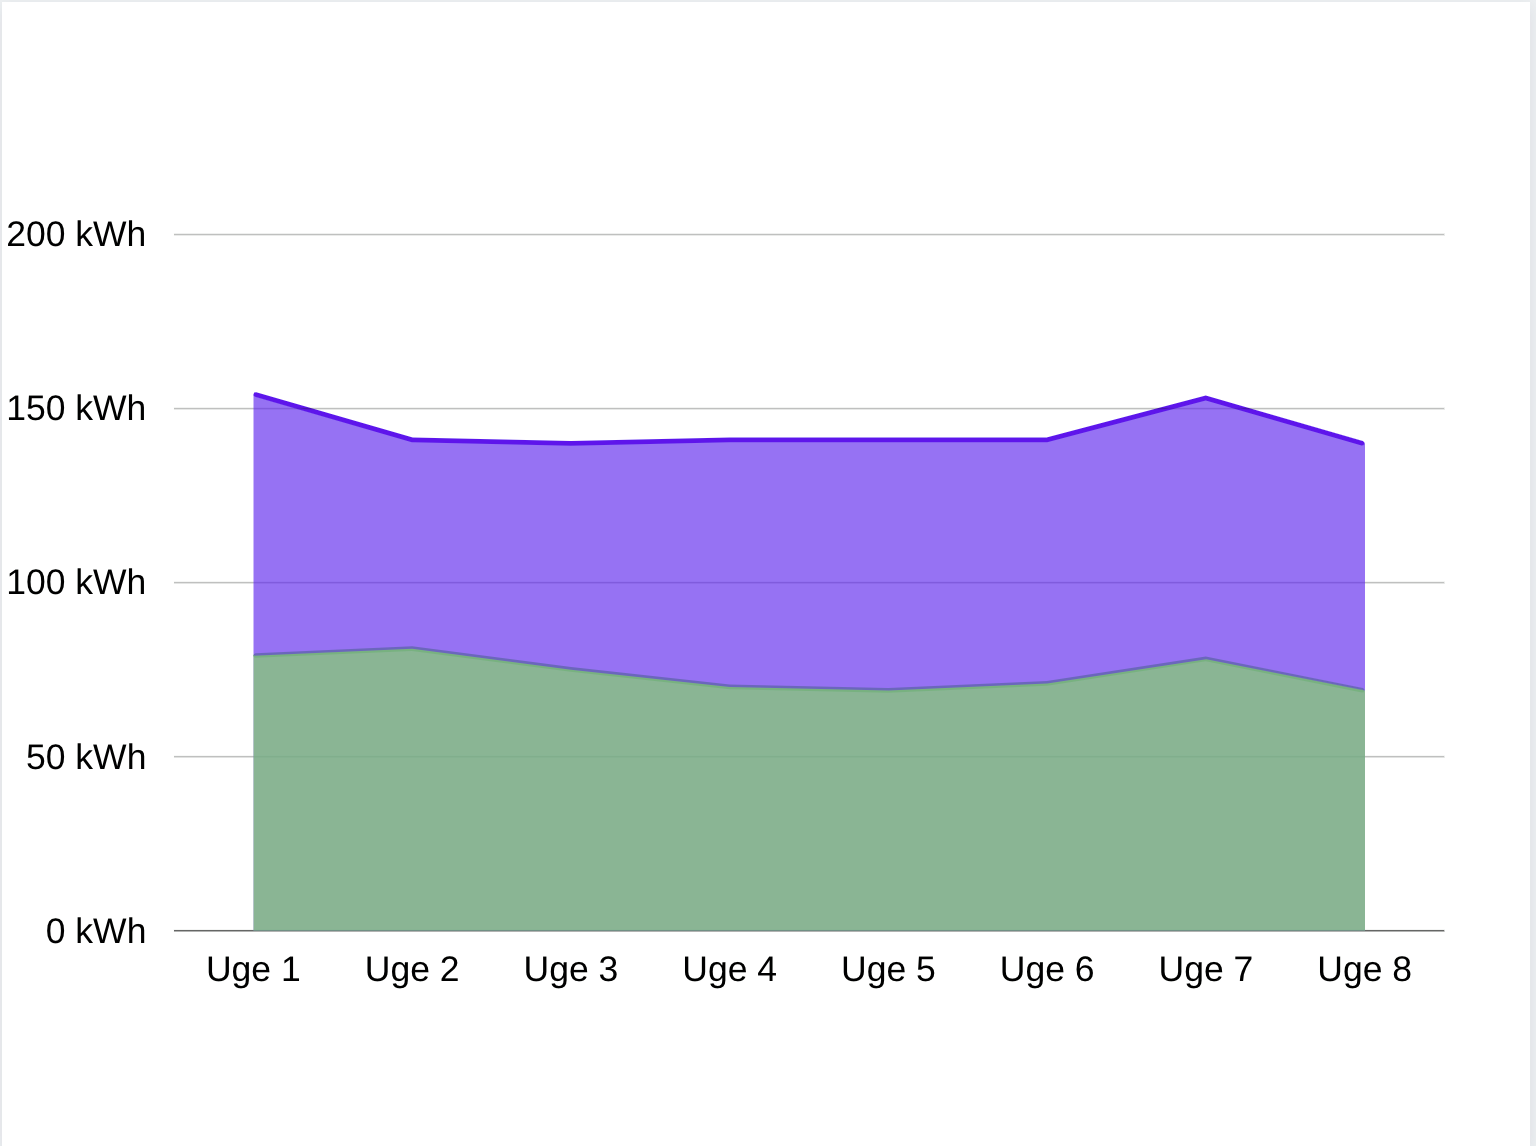
\includegraphics[width=\textwidth]{Images/appendixA/graph.png}
        \caption[Graf 1 til spørgeskema del 3]{Med i spørgsmål: 3a og 3b}
    \end{subfigure}
    \hfill
    \begin{subfigure}[b]{0.45\textwidth}
        \centering
        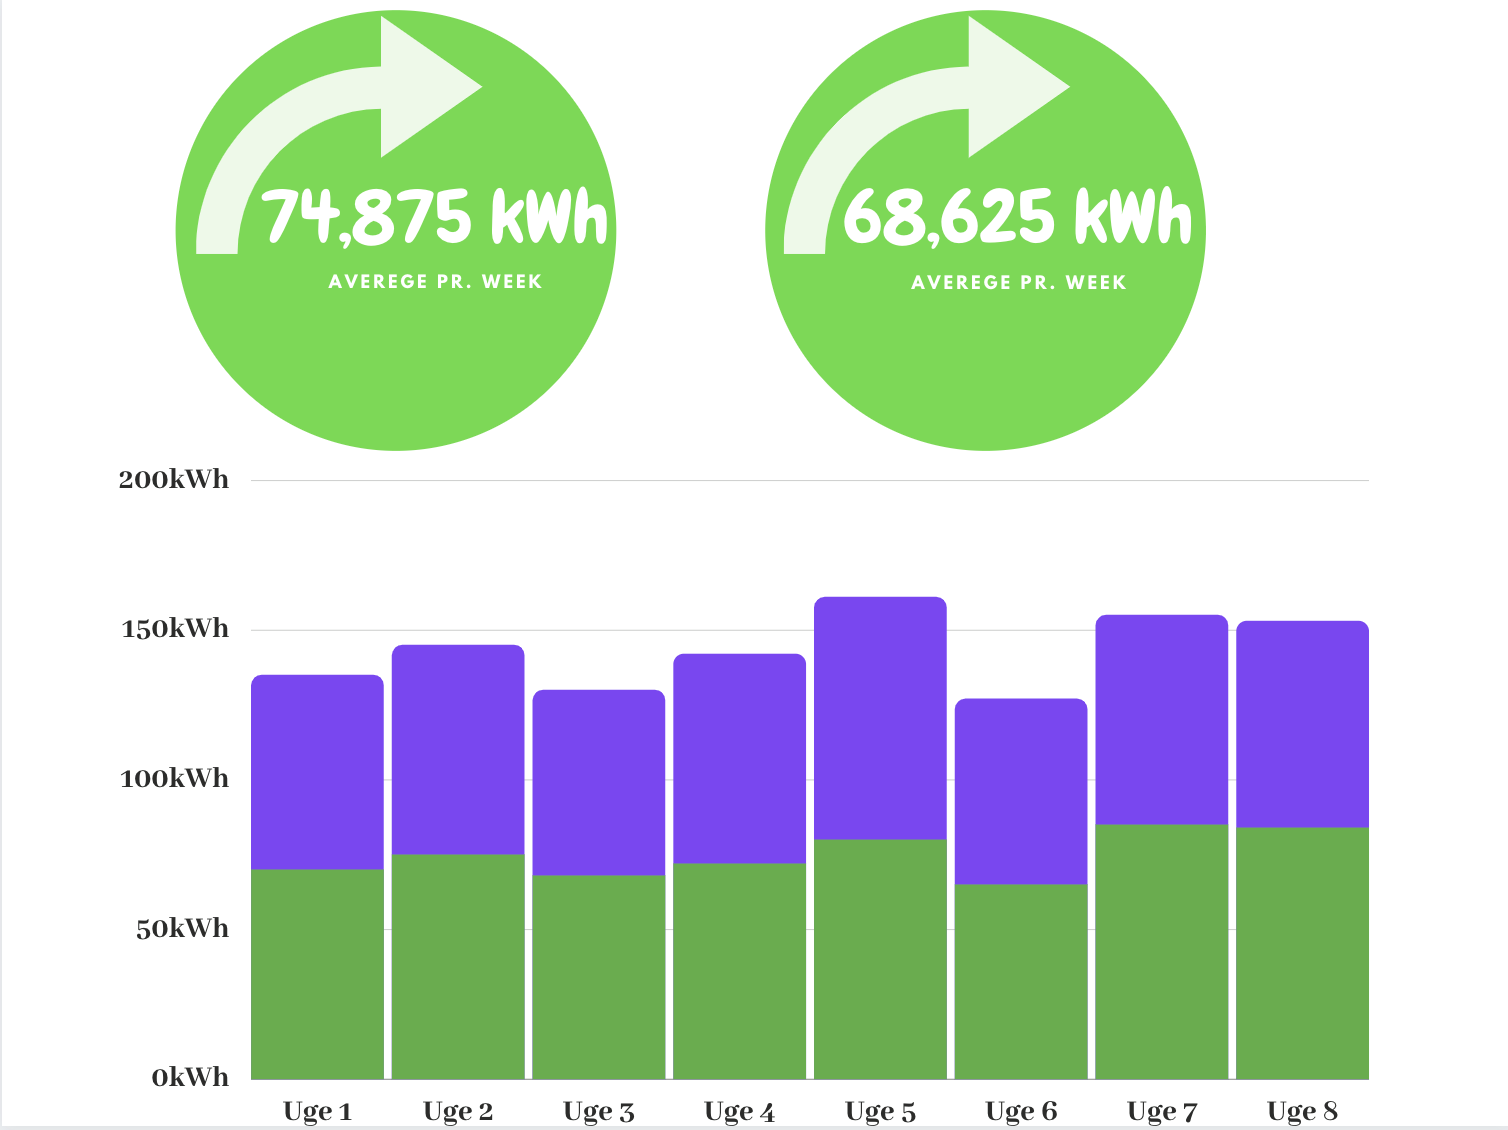
\includegraphics[width=\textwidth]{Images/appendixA/hist_wheel.png}
        \caption[Graf 2 til spørgeskema del 3]{Med i spørgsmål: 3d}
    \end{subfigure}
    \hfill
    \begin{subfigure}[b]{0.45\textwidth}
        \centering
        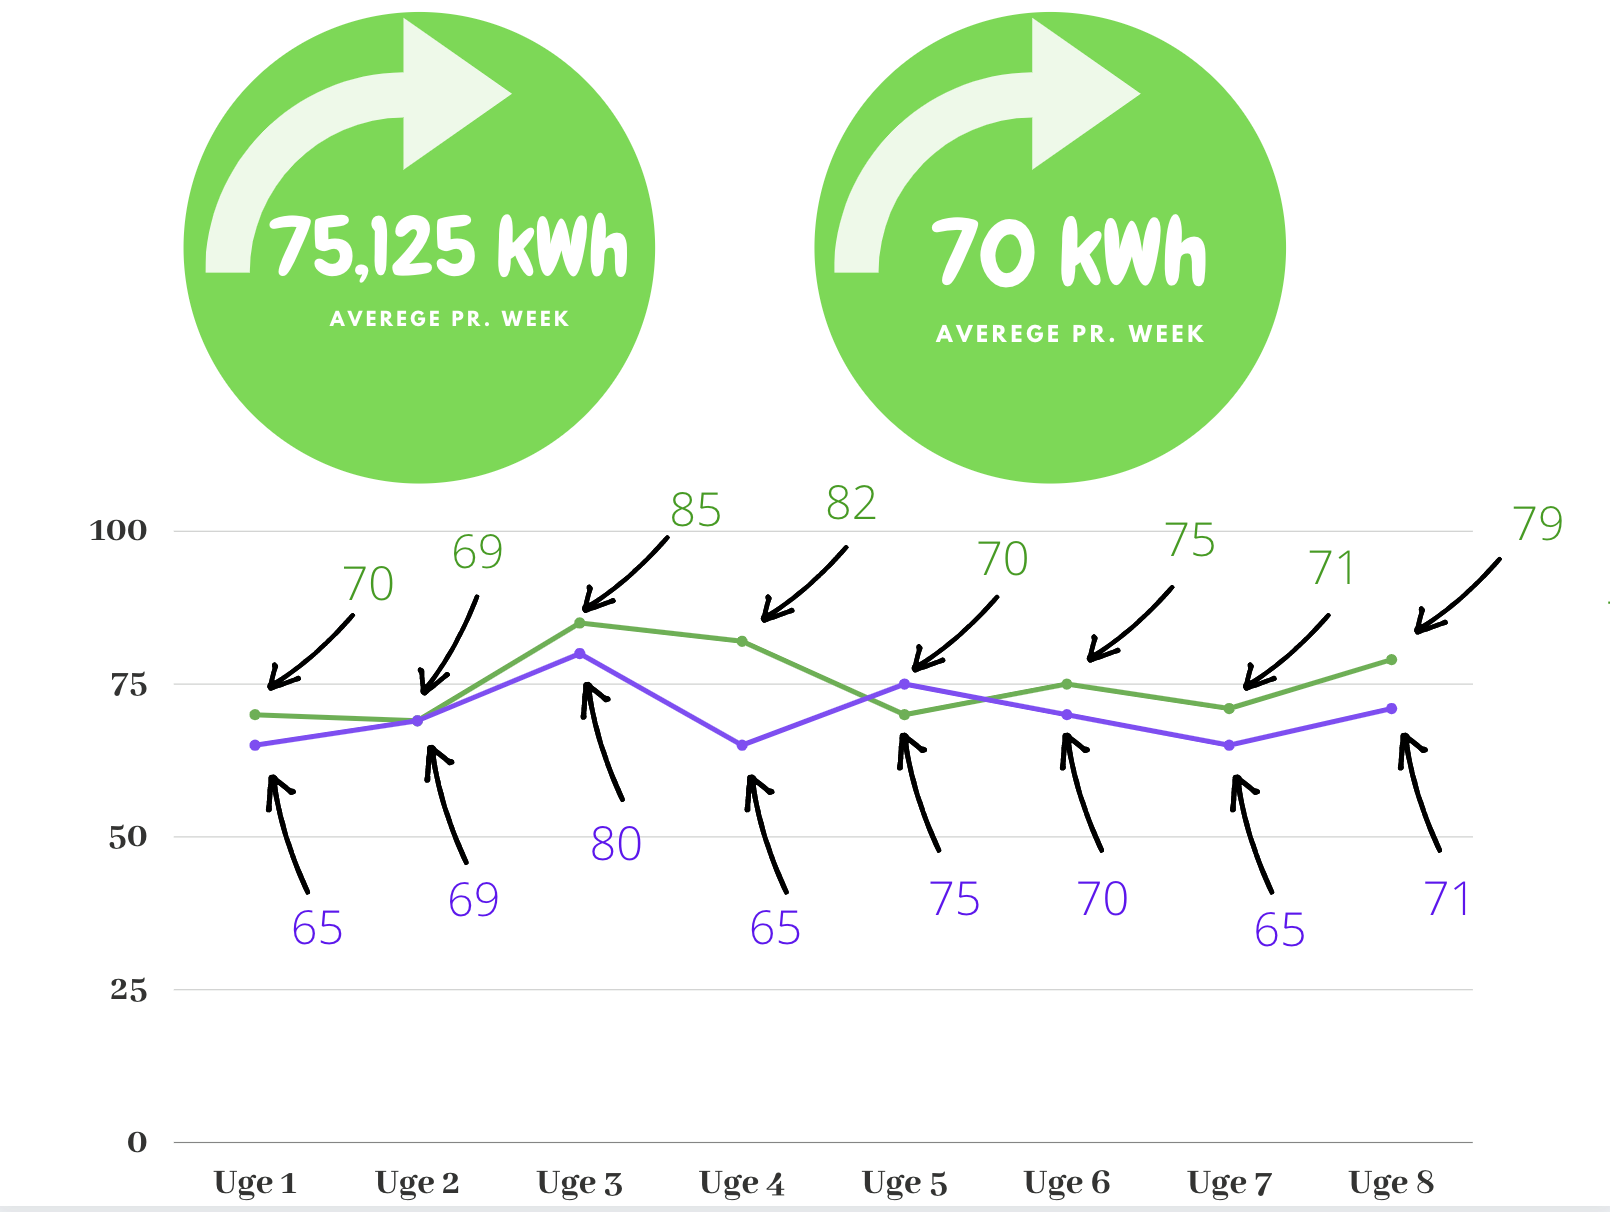
\includegraphics[width=\textwidth]{Images/appendixA/num_wheel.png}
        \caption[Graf 3 til spørgeskema del 3]{Med i spørgsmål: 3e, 3f og 3g}
    \end{subfigure}
    \hfill
    \begin{subfigure}[b]{0.45\textwidth}
        \centering
        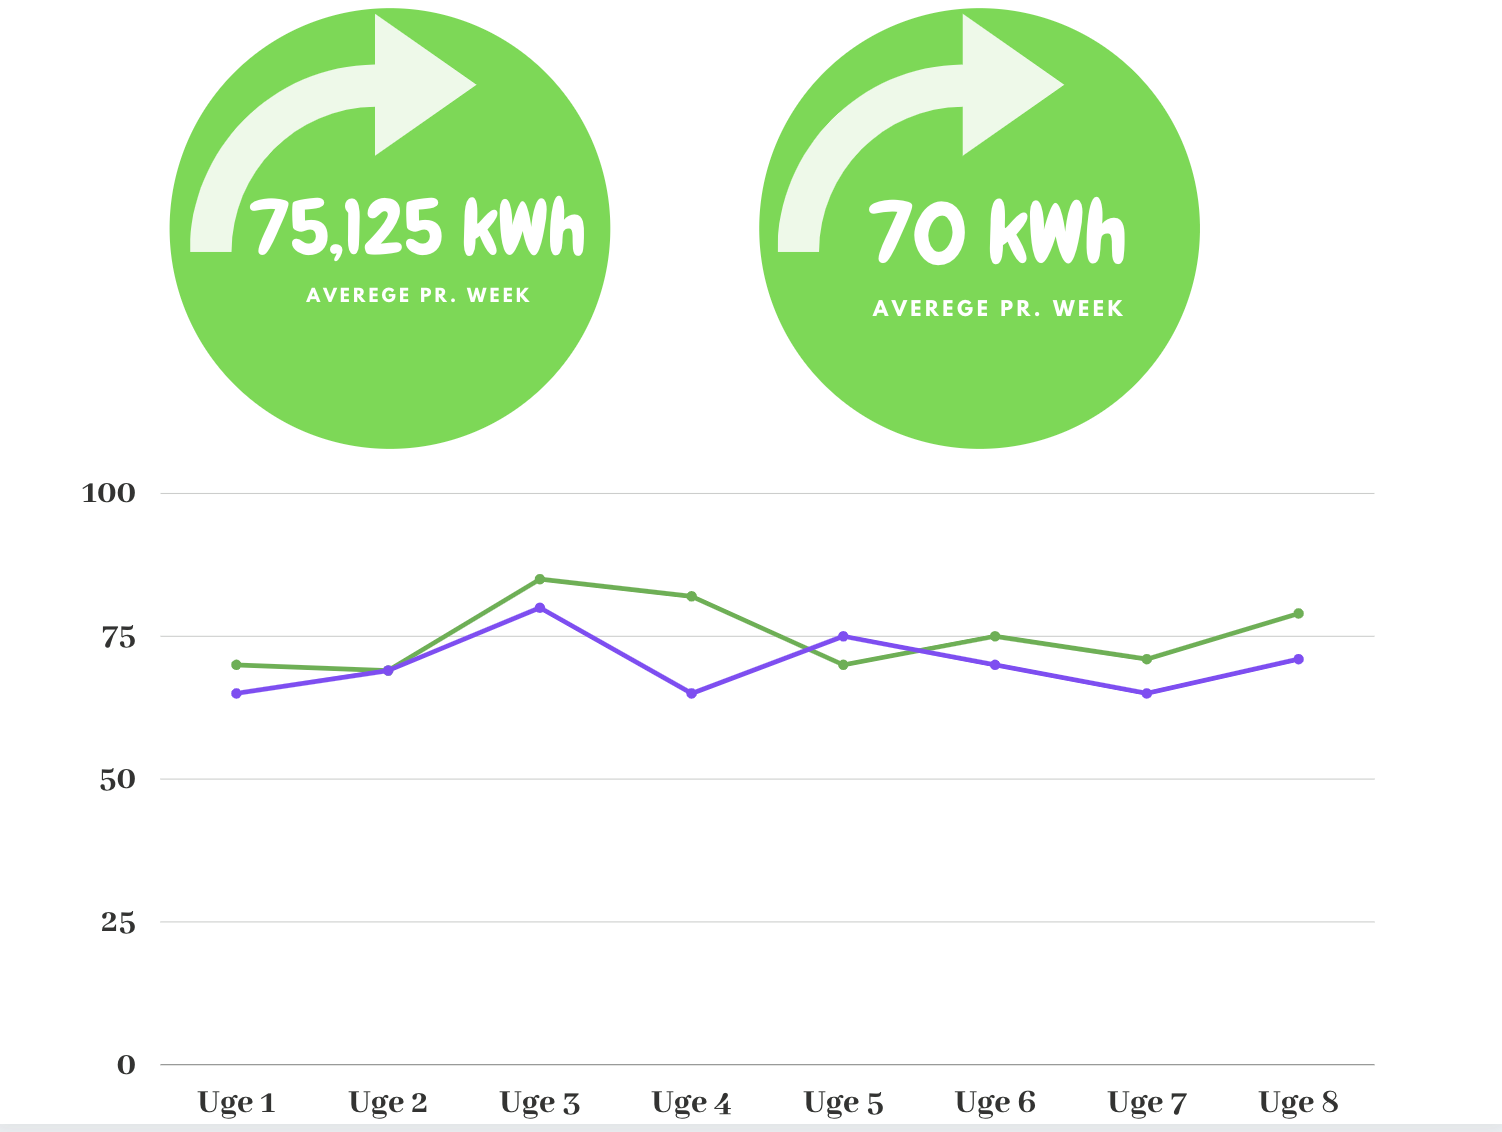
\includegraphics[width=\textwidth]{Images/appendixA/wheel.png}
        \caption[Graf 4 til spørgeskema del 3]{Med i spørgsmål: 3c}
    \end{subfigure}
    \caption{Grafer til del 3 af spørgeskemaet}
    \label{fig:survey:graphs1}
\end{figure}
\begin{figure}[H]
    \centering
    \begin{subfigure}[b]{0.45\textwidth}
        \centering
        \includegraphics[width=\textwidth]{Images/appendixA/Grafer og data-grafik til undersøgelser-04.png}
        \caption[Graf 1 til spørgeskema del 4]{Med i spørgsmål: 4a, 4b, 4c og 4d}
    \end{subfigure}
    \hfill
    \begin{subfigure}[b]{0.45\textwidth}
        \centering
        \includegraphics[width=\textwidth]{Images/appendixA/Grafer og data-grafik til undersøgelser-05.png}
        \caption[Graf 2 til spørgeskema del 4]{Med i spørgsmål: 4e og 4f}
    \end{subfigure}
    \hfill
    \begin{subfigure}[b]{0.45\textwidth}
        \centering
        \includegraphics[width=\textwidth]{Images/appendixA/Grafer og data-grafik til undersøgelser-07.png}
        \caption[Graf 3 til spørgeskema del 4]{Med i spørgsmål: 4g}
    \end{subfigure}
    \hfill
    \begin{subfigure}[b]{0.45\textwidth}
        \centering
        \includegraphics[width=\textwidth]{Images/appendixA/Grafer og data-grafik til undersøgelser-06.png}
        \caption[Graf 4 til spørgeskema del 4]{Med i spørgsmål: 4h}
    \end{subfigure}
    \hfill
    \begin{subfigure}[b]{0.45\textwidth}
        \centering
        \includegraphics[width=\textwidth]{Images/appendixA/Grafer og data-grafik til undersøgelser-02.png}
        \caption[Graf 5 til spørgeskema del 4]{Med i spørgsmål: 4i, 4j og 4k}
    \end{subfigure}
    \caption{Grafer til del 4 af spørgeskemaet}
    \label{fig:survey:graphs2}
\end{figure}

\section{Spørgsmål og svar}
For at holde brugeren i gang så er svar mulighederne på multiple choice spørgsmålene, i tilfældig rækkefølge når brugeren skal svare.\\
Svarene vil være i formatet, "Hvor mange der svarede det" - "Hvad det svar var"
\subsection{Information om dig}
\subsubsection{Hvor gammel er du?}
\textbf{Svar}
\begin{itemize}
    \item 5 - 20
    \item 5 - 21
    \item 7 - 22
    \item 4 - 23
    \item 1 - 24
    \item 1 - 25
    \item 1 - 26
    \item 1 - 27
    \item 1 - 28
    \item 1 - 33
    \item 1 - 34
    \item 1 - 37
    \item 1 - 40
    \item 2 - 45
    \item 1 - 47
    \item 2 - 49
    \item 1 - 50
    \item 1 - 56
    \item 1 - 59
    \item 1 - 62
    \item 1 - 71
\end{itemize}

\subsubsection{Hvilken stilling er du i? Hvis du er studerende, hvilken uddannelse?}
\textbf{Svar}
\begin{itemize}
    \item 5 - Sygeplejerske
    \item 13- Softwareudvikling
    \item 1 - Lægesekretær
    \item 1 - HA EUROPEAN BUSINESS
    \item 1 - Kontor arbejde
    \item 1 - Msc. Computer Science
    \item 1 - Digital design og interaktive teknologier
    \item 1 - IT seniorkonsulent
    \item 1 - Ingeniør
    \item 1 - Studerende
    \item 1 - Lukkeansvarlig i en Irma
    \item 1 - Ssa
    \item 1 - Underviser
    \item 1 - Pensionist
    \item 1 - Sygemeldt
    \item 1 - Supplering: Fysik 0-B
    \item 1 - SamTek - Miljøplanlægning, RUC
    \item 1 - Afd.sygeplejerske
    \item 1 - Sundhedsteknologi på AU
    \item 1 - Projektledelse
    \item 1 - Elev
    \item 1 - Konsulent
    \item 1 - Lærer
    \item 1 - Timelønnet
\end{itemize}

\subsection{I konteksten af et smart hjem, hvilken data vil du gerne have?}
\textbf{Svar}
\begin{itemize}
    \item 1 - Mit forburg
    \item 1 - Besparelser/ overforbrug
    \item 2 - Besparelse
    \item 1 - Energiforbrug, indeklima
    \item 1 - Mængde af soltimer
    \item 1 - nan
    \item 1 - Hvor meget data jeg bruger, hvem der tilgår mine devices, strømforbrug af forskellige appliances.
    \item 1 - Energibesparelse
    \item 1 - Alt vedr. forbrug: el, gas, vand. Indeklima: temperatur, fugtighed, og hvad ellers kunne blive relevant
    \item 1 - Kan ikke komme på andet end det i har nævnt
    \item 1 - kW forbrug, fugtighed og indeklima. Alternativt, lokalt vejr- og trafikoverblik.
    \item 1 - Temperatur, indeklima, fugtighed, røgalarm, overvågning.
    \item 1 - kWh
    \item 1 - Elforbrug og forslag til at spare mere på forbruget. Måling af luft og indhold af skadelige partikler
    \item 1 - Det hele
    \item 1 - Hvad der bliver brugt, og hvor ofte, samt hvad jeg kunne spare på.
    \item 1 - El forbrug.  Fugt i bolig.
    \item 1 - Indeklima
    \item 1 - Indeklima såsom f.eks fugt, radon, skimmel m.m. Energiforbrug såsom strøm, vand og varme.
    \item 1 - Hvordan skulle jeg vide det?
    \item 1 - Fugtighed og gas
    \item 1 - Sensor af indeklima i forhold til allergi, fugt, røg. Udluftning der lukker hvis tobaksrøg og grillrøg kommer ind udefra fra naboer.
    \item 1 - Alle de ovenstående
    \item 1 - Grøn energi
    \item 1 - Intet
    \item 1 - Alt
    \item 1 - Primært oplysninger om forbrug som vand, el, gas, og fjerenvarme. Dertil kunne det måske opdeles i rum, sådan at man kan se at dagligstuen bruger denne mængde energi til varme, hvorimod soveværelset bruger en anden mængde. Som tilføjelse kunne dataen præsenteres i forbindelse med tid, så man kan få overblik over sit på forbrug på forskellige tidspunkter.
    \item 1 - Tid for hvor lang tid ting har været tændt. Data for, hvornår på dagen forskellige ting bliver brugt mest. Hvor I hjemmet, der bruges mest strøm.
    \item 1 - Forbrug af el, varme, nem adgang til udsving i forbrug, lokation af el forbrug pr rum, pr beboer, temp osv
    \item 1 - kilowatt forbrug, indeklima og fugtighed hovedsageligt
    \item 1 - Med stikkontakter ville jeg gerne kunne se hvilke af dem der var i brug, altså hvilke der er tændt og bruger strøm. Indeklima sensor gad jeg gerne vide temperaturen.
    \item 1 - Indeklima, mulige besparelser, forbrug i løbet af dagen
    \item 1 - Alarmer, forbrug og priser/besparelse
    \item 1 - Varmebesparelser, varmeforbrug, vandforbrug, fugtighed,
    \item 1 - Kilowatt-forbrug og gasser
    \item 1 - Forbrug - evt advarsler om merforbrug af f.eks vand og el.
    \item 1 - Besparelse og smarte kontakter
    \item 1 - Besparelse og kilowatt forbrug
    \item 1 - Kilowatt forbrug, Indeklima
\end{itemize}

\subsection{Data visualisering - Forskel}
\subsubsection{Ca. Hvor stor en ændring mellem datapunkterne var der i uge 2}
\textbf{Svar muligheder}
\begin{itemize}
    \item ~55 kWh
    \item ~65 kWh
    \item ~75 kWh
    \item ~90 kWh
\end{itemize}

\textbf{Svar}
\begin{itemize}
    \item 8 - ~55 kWh
    \item 12 - ~65 kWh
    \item 15 - ~75 kWh
    \item 5 - ~90 kWh
\end{itemize}

\subsubsection{Ca. Hvor stor en ændring mellem datapunkterne var der i uge 6}
\textbf{Svar muligheder}
\begin{itemize}
    \item ~50 kWh
    \item ~55 kWh
    \item ~60 kWh
    \item ~65 kWh
    \item ~70 kWh
    \item ~75 kWh
    \item ~90 kWh
\end{itemize}

\textbf{Svar}
\begin{itemize}
    \item 4 - ~50 kWh
    \item 5 - ~65 kWh
    \item 13 - ~70 kWh
    \item 9 - ~75 kWh
    \item 4 - ~55 kWh
    \item 3 - ~60 kWh
    \item 2 - ~90 kWh
\end{itemize}

\subsubsection{Hvilken uge var der den største ændring mellem datasættene}
\textbf{Svar muligheder}
\begin{itemize}
    \item Uge 1
    \item Uge 2
    \item Uge 3
    \item Uge 4
    \item Uge 5
    \item Uge 6
    \item Uge 7
    \item Uge 8
\end{itemize}

\textbf{Svar}
\begin{itemize}
    \item 2 - Uge 3
    \item 36 - Uge 4
    \item 1 - Uge 1
    \item 1 - Uge 5
\end{itemize}

\subsubsection{Hvor stor er ændringen af gennemsnittet mellem de to datasæt}
\textbf{Svar muligheder}
\begin{itemize}
    \item ~5.25 kWh
    \item ~5.50 kWh
    \item ~6.25 kWh
    \item ~6.50 kWh
    \item ~6.75 kWh
    \item ~7.00 kWh
\end{itemize}

\textbf{Svar}
\begin{itemize}
    \item 5 - ~7.00 kWh
    \item 5 - ~6.75 kWh
    \item 14 - ~6.25 kWh
    \item 5 - ~5.50 kWh
    \item 4 - ~5.25 kWh
    \item 6 - ~6.50 kWh
\end{itemize}

\subsubsection{Hvor stor er forskellen mellem datapunkterne i uge 5?}
\textbf{Svar muligheder}
\begin{itemize}
    \item 2
    \item 3
    \item 4
    \item 5
    \item 6
    \item 7
    \item 8
\end{itemize}

\textbf{Svar}
\begin{itemize}
    \item 37 - 5
    \item 1 - 3
    \item 1 - 4
    \item 1 - 6
\end{itemize}

\subsubsection{Hvor stor er forskellen mellem datapunkterne i uge 7?}
\textbf{Svar muligheder}
\begin{itemize}
    \item 3
    \item 4
    \item 5
    \item 6
    \item 7
    \item 8
    \item 9
\end{itemize}

\textbf{Svar}
\begin{itemize}
    \item 34 - 6
    \item 3 - 5
    \item 1 - 9
    \item 2 - 4
\end{itemize}

\subsubsection{Hvilken uge var der ikke en ændring i datasættene?}
\textbf{Svar muligheder}
\begin{itemize}
    \item Uge 1
    \item Uge 2
    \item Uge 3
    \item Uge 4
    \item Uge 5
    \item Uge 6
    \item Uge 7
    \item Uge 8
\end{itemize}

\textbf{Svar}
\begin{itemize}
    \item 35 - Uge 2
    \item 1 - Uge 6
    \item 2 - Uge 7
    \item 1 - Uge 4
    \item 1 - Uge 8
\end{itemize}

\subsubsection{Hvilken af de 5 grafer er det nemmest at aflæse værdien i en bestemt uge? Skriv gerne hvorfor.}
\textbf{Svar}
\begin{itemize}
    \item 1 - der er ingen legende, jeg kan ikke læse nogen af dem
    \item 1 - 4
    \item 1 - 1 - lettest at overskue
    \item 1 - Nr 5
    \item 1 - Nr 3 der er værdier på
    \item 2 - nan
    \item 1 - 3, præcise tal.
    \item 13 - 5
    \item 1 - Tredje graf, dog burde tallene på selve grafen være lidt mere nedtonede
    \item 1 - Den femte. Tallene er tydelige, og har god plads i mellem så det er nemt at aflæse.
    \item 1 - Sidste - forskel er tydelig fra uge til uge
    \item 1 - Mere logisk. Der “sker” ikke så meget i billedet
    \item 1 - 3,4 eller 5
    \item 1 - 5 der er tal tydeligst
    \item 1 - Øverst til venstre
    \item 2 - 3
    \item 1 - 5 fordi tallene er skrevet og man ikke skal bruge øjemål over til tallene i venstre side
    \item 1 - nummer 5 fordi der var tal til den individuelle uge
    \item 1 - 5, fordi tallet står der. Men generelt burde der nok være flere "mellemstreger" til lettere aflæsning (i stedet for kun ved 50, 100, 150)
    \item 1 - Måske 1, Synes de alle gir et visuelt overblik men man gætter den egentlige værdi på data
    \item 1 - Den hvor der står precise tal på, så nr 5
    \item 1 - Der hvor tallene står på kurven med en pil
    \item 1 - 1
    \item 1 - Helt klart nr. 5, da der kom konkrete tal på bordet. Det kunne smart, hvis man just kunne holde på den, og så man fik den konkrete info
    \item 1 - Overskuelig
    \item 1 - 5, Den er klart nemmest at læse! Hver punkts tal hjælper meget
\end{itemize}

\subsubsection{Hvilken af de 5 grafer giver hurtigst overblik over dit forbrug? Skriv gerne hvorfor.}
\textbf{Svar}
\begin{itemize}
    \item 1 - 4 eller 5 tror jeg
    \item 5 - 1
    \item 1 - Nr 4
    \item 1 - Stadig 3 der er værdier
    \item 5 - nan
    \item 1 - 3, jeg kan rent faktisk se tallene.
    \item 6 - 5
    \item 1 - 5, tallene står der direkye
    \item 1 - Tredje og femte da du hurtigt kan se hvor der er store ændringer
    \item 1 - 5, kræver ikke aflæsning af akserne. Men der mangler lidt lodret grid streger
    \item 1 - Det er nemmere at se forskellen mellem de to data i nr.5
    \item 1 - Den anden. Det er nemt at se hvilken der er uge har den højeste/laveste værdi
    \item 1 - 5 der er tal og graf tydeligst
    \item 1 - 5. Umiddelbart virker tydeligheden af tallene mere overskueligt
    \item 1 - Øverst til venstre, den er tydligst og mest menneskenær
    \item 5 - 2
    \item 1 - 5. Vandret er godt og godt at tallene er skrevet
    \item 2 - 3
    \item 1 - 2, fordi man er vant til at læse et klassisk søjlediagram
    \item 1 - 4 - jeg har brug for et hurtigt overblik der grafisk fortæller hvad jeg har brugt. Jeg har ikke brug for den detaljerede
    \item 1 - 2 eller 5. De har begge gennemsnitsmåler, og det er nemt at sammenligne
    \item 1 - 4
\end{itemize}

\subsubsection{På hvilken af de 5 grafer er det nemmest at aflæse forskellen mellem to datasæt? Skriv gerne hvorfor.}
\textbf{Svar}
\begin{itemize}
    \item 1 - 4 og 5 fordi de ikke er stablet
    \item 1 - 5 - skrevne tal
    \item 1 - 1
    \item 1 - Nr 4
    \item 1 - Jeg har skrevet forket har ikke kunne se tallene
    \item 1 - Nr 3 fordi der er angivet tal
    \item 1 - 3 igen, jeg kan se de konkrette tal.
    \item 13 - 5
    \item 1 - 5, du skal bare trække 2tal fra hinanden
    \item 1 - Den tredje da mellemrummet mellem dem er forskellen
    \item 1 - 5,samme som forrige spørgsmål
    \item 1 - Den fjerde. At have de to grafer "oven på" hinanden gør det meget nemt at sammenligne.
    \item 1 - Sidste
    \item 1 - nan
    \item 1 - 4
    \item 1 - Øverst til venstre
    \item 3 - 3
    \item 1 - 5 fordi der står tallene og graferne er tydelige
    \item 1 - 5 igen på grund af datapunkterne
    \item 1 - 2
    \item 1 - 3. Da graferne er adskilte
    \item 1 - 5, for der er præcise tal
    \item 1 - Nr. 5 - værdierne står på kurven
    \item 1 - 5 - er klart nemmest hvis du snakker detaljer. 4 tænker jeg er mere brugervenligt.
    \item 1 - Nr. 5, pga overblik og komkrethed
    \item 1 - 5 fordi man ser hver punkts værdi
\end{itemize}

\subsection{Data visualisering - Data}
\subsubsection{Hvor mange uger blev der undersøgt?}
\textbf{Svar muligheder}
\begin{itemize}
    \item 4
    \item 6
    \item 7
    \item 8
\end{itemize}

\textbf{Svar}
\begin{itemize}
    \item 39 - 8.0
\end{itemize}

\subsubsection{Hvor meget var forbruget i uge 1?}
\textbf{Svar muligheder}
\begin{itemize}
    \item 300
    \item 400
    \item 500
\end{itemize}

\textbf{Svar}
\begin{itemize}
    \item 37 - 500.0
    \item 1 - 300.0
    \item 1 - 400.0
\end{itemize}

\subsubsection{I hvor mange uger var forbruget over 500?}
\textbf{Svar muligheder}
\begin{itemize}
    \item 4
    \item 5
    \item 6
    \item 7
    \item 8
\end{itemize}

\textbf{Svar}
\begin{itemize}
    \item 28 - 5.0
    \item 11 - 4.0
\end{itemize}

\subsubsection{I hvilken uge var forbruget størst?}
\textbf{Svar muligheder}
\begin{itemize}
    \item 4
    \item 5
    \item 6
    \item 7
    \item 8
\end{itemize}

\textbf{Svar}
\begin{itemize}
    \item 38 - Uge 7
    \item 2 - Uge 4
\end{itemize}

\subsubsection{Hvad var det samlede forbrug for uge 2 til uge 4?}
\textbf{Svar}
\begin{itemize}
    \item 6 - 1500.0
    \item 1 - 8.0
    \item 1 - 850.0
    \item 8 - 1550.0
    \item 3 - 1600.0
    \item 2 - 1400.0
    \item 1 - 780.0
    \item 1 - 1420.0
    \item 1 - 600.0
    \item 2 - 200.0
    \item 1 - 1575.0
    \item 1 - 500.0
    \item 1 - 1585.0
    \item 2 - 400.0
    \item 1 - 720.0
    \item 1 - 1650.0
    \item 1 - 1475.0
    \item 1 - 750.0
    \item 2 - 800.0
\end{itemize}

\subsubsection{Hvad var det gennemsnitlige forbrug for uge 4 til uge 7?}
\textbf{Svar}
\begin{itemize}
    \item 1 - 1500.0
    \item 1 - 50.0
    \item 1 - 9.0
    \item 2 - 250.0
    \item 1 - 675.0
    \item 7 - 400.0
    \item 1 - 1600.0
    \item 2 - 350.0
    \item 1 - 525.0
    \item 1 - 1400.0
    \item 1 - 930.0
    \item 1 - 0.0
    \item 3 - 300.0
    \item 1 - 110.0
    \item 1 - 900.0
    \item 1 - 1465.0
    \item 7 - 500.0
    \item 1 - 1350.0
    \item 1 - 240.0
    \item 1 - 450.0
    \item 1 - 220.0
    \item 1 - 750.0
    \item 1 - 625.0
\end{itemize}

\subsubsection{Hvad var det samlede forbrug for uge 3 til uge 4?}
\textbf{Svar}
\begin{itemize}
    \item 1 - 1500.0
    \item 1 - 1100.0
    \item 1 - 5.0
    \item 9 - 1400.0
    \item 1 - 575.0
    \item 1 - 2200.0
    \item 1 - 1300.0
    \item 5 - 1450.0
    \item 2 - 1350.0
    \item 1 - 1475.0
    \item 1 - 750.0
    \item 1 - 125.0
    \item 3 - 1437.0
    \item 1 - 200.0
    \item 1 - 130.0
    \item 1 - 700.0
    \item 1 - 1250.0
    \item 1 - 550.0
    \item 2 - 800.0
    \item 2 - 400.0
    \item 1 - 1200.0
    \item 1 - 2000.0    
\end{itemize}

\subsubsection{Hvad var det samlede forbrug for uge 3 til uge 6, i den blå graf?}
\textbf{Svar}
\begin{itemize}
    \item 1 - 2100.0
    \item 1 - 3500.0
    \item 1 - 0.0
    \item 11 - 2567.0
    \item 1 - 2650.0
    \item 2 - 2400.0
    \item 2 - 1300.0
    \item 1 - 2600.0
    \item 1 - 2550.0
    \item 2 - 2500.0
    \item 1 - 1470.0
    \item 1 - 23.0
    \item 1 - 600.0
    \item 1 - 1450.0
    \item 2 - 1807.0
    \item 1 - 1443.0
    \item 1 - 1810.0
    \item 2 - 2560.0
    \item 1 - 1800.0
    \item 1 - 200.0
    \item 1 - 750.0
    \item 1 - 1520.0
\end{itemize}

\subsubsection{Hvad var det samlede forbrug for uge 4 til uge 7, i den røde graf?}
\textbf{Svar}
\begin{itemize}
    \item 2 - 2400.0
    \item 1 - 1700.0
    \item 1 - 100.0
    \item 12 - 2612.0
    \item 1 - 0.0
    \item 1 - 2700.0
    \item 1 - 2300.0
    \item 2 - 1100.0
    \item 1 - 1500.0
    \item 1 - 2550.0
    \item 1 - 2500.0
    \item 1 - 160.0
    \item 1 - 650.0
    \item 2 - 1140.0
    \item 1 - 1962.0
    \item 2 - 2600.0
    \item 1 - 2650.0
    \item 1 - 2524.0
    \item 1 - 220.0
    \item 1 - 2000.0
    \item 1 - 400.0
    \item 1 - 830.0
    \item 1 - 2430.0
    \item 1 - 3120.0    
\end{itemize}

\subsubsection{Hvad var det gennemsnitlige forbrug for uge 4 til uge 7, i den røde graf?}
\textbf{Svar}
\begin{itemize}
    \item 1 - 2400.0
    \item 1 - 1960.0
    \item 1 - 20.0
    \item 8 - 653.0
    \item 1 - 0.0
    \item 1 - 670.0
    \item 1 - 2500.0
    \item 1 - 1100.0
    \item 3 - 700.0
    \item 1 - 1900.0
    \item 2 - 2612.0
    \item 2 - 600.0
    \item 1 - 620.0
    \item 1 - 160.0
    \item 1 - 900.0
    \item 1 - 1306.0
    \item 1 - 2.0
    \item 3 - 500.0
    \item 1 - 2567.0
    \item 1 - 575.0
    \item 2 - 650.0
    \item 1 - 662.0
    \item 1 - 10.0
    \item 1 - 640.0
    \item 1 - 750.0    
\end{itemize}
